\documentclass{article}

\usepackage[english]{babel}
\usepackage[a4paper,top=2cm,bottom=2cm,left=3cm,right=3cm,marginparwidth=1.75cm]{geometry}
\usepackage{amsmath}
\usepackage{enumitem}
\usepackage{graphicx}
\usepackage[colorlinks=true, allcolors=blue]{hyperref}
\usepackage[super]{nth}

\newcommand{\todo}[1]{\textcolor{red}{TODO: #1}}

\title{Multi-Agent Systems Lab - Report 3}
\author{Group 7}

\begin{document}
\maketitle

\begin{enumerate}

\item \textbf{Introducing Agent 007} - This is an agent that wants to find the best possible agreement and is actively searching for it. This can be seen in the bidding strategy, where it tries to find bids that are great for itself and also decent for the opponent, which should be a point close to the Pareto-optimal frontier. This is only possible if there is enough knowledge about the opponent. Therefore, we only start actually offering these types of bids after the agent know enough about the opponent (we believe this threshold is crossed when the last updates to our opponent model no longer change it drastically). The opponents preferences are being modelled by a Bayesian model, which updates after every bid it receives. 

Another component that should be highlighted is the acceptance strategy. It tries to find when a good deal is being offered, while still maintaining high standards. This especially happens at the beginning, since it wants to give the bidding strategy time to find bids that are close to the Pareto-optimal frontier and find a bid with high utility for both agents. All these components will be explained in further detail in the next couple of sections.

\item \textbf{NEGOTIATION STRATEGY IMPLEMENTATION}

\begin{itemize}

\item \textbf{Acceptance Strategy}: The acceptance strategy indicates whether or not the agent should accept the opponent's bid. Agent 007's acceptance strategy depends on both the time remaining and the utility of the offers, since having both components could help it increase the performance \cite{baarslag}. The time component is essential because both agents are incentivized to reach an agreement, else both agents would get an utility of 0. The acceptance of the opponents bid will depend on multiple issues which will be covered in the next sections. At the early stages of the negotiation the utility of an opponents bid needs to be very high for it to be accepted, because for the beginning of the negotiation, which can last up to 60 percent of the total time, the agent is getting to know the opponent negotiator. In the first phase, the preferences of the opponent are getting modelled with help of the opponent Bayesian modeling.

After this phase, the acceptance utility goes down in a certain fashion. It will go down parabolically to a certain endpoint, and thus it will decrease at a faster rate when the deadline is closer, otherwise the agent would accept an offer while it could have gotten a better offer in the future. At each time-step the acceptance utility decreases with a certain amount which is connected to the decline rate. This decline rate is being calculated by using a starting point and the endpoint. The endpoint is the lowest utility our agent is willing to accept at the end of the negotiation. This endpoint is chosen to start at the average utility of all bids in the current domain. This first endpoint has been chosen because it takes into account the utilities in a domain. Thus our agent is now more dynamic since its acceptance strategy is changing depending on the domain. This endpoint can be set higher if certain criteria are met. This process is showed in Figure \ref{fig:acceptance} and can happen multiple times in a negotiation.

\begin{figure}[h!]
    \centering
    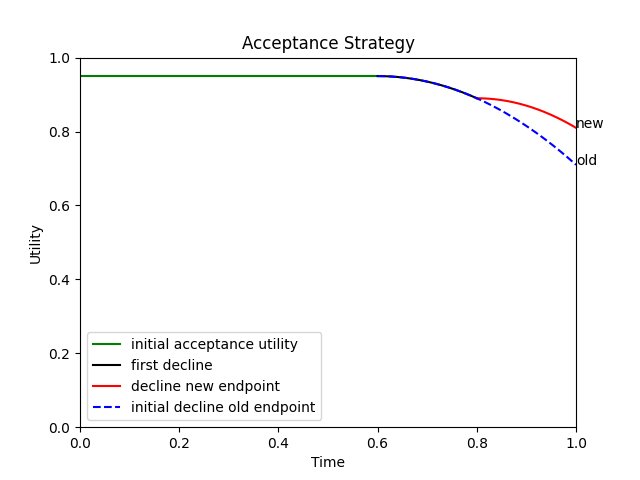
\includegraphics[width=280pt]{acceptance_strat.png}
    \caption{A clear case where the endpoint shifts to a new higher place. all bids that are above the line will be accepted. }
    \label{fig:acceptance}
\end{figure}

The endpoint is set higher when the utility of an opponent's bid is higher then the previous set endpoint. Thus there will be a new endpoint with this former mentioned utility. The agent now knows that the opponent is capable of bidding a bid with a higher utility than the endpoint, thus if the endpoint was kept the same then the acceptance utility could go lower then the utility of an opponent's previous bid. The endpoint should thus be set higher so that the agent will never accept offers that are lower than a previous offer the opponent has made.

There is a second way for the endpoint to shift which includes the modelling of our utility of the opponent's bid. This modelling was done with the help of the method least squares regression which finds the best fit of a line through the data points. The slope of this line has been found by using the formula below where x is the time and y the utility.

\[ slope = \frac { \Sigma (x-\bar{x} )(y-\bar{y} )} {\Sigma (x- \bar{x} )^2} \]

This line was used to find the endpoint at the end of the time of the negotiation. If this endpoint was higher than the previous set endpoint then it replaces it. Thus this entails that if we expect the opponent to place a bid with a higher utility in the future then we should wait for it and thus change the acceptance utility accordingly. This method has its use when the utility of the opponent's bids go up in a linear fashion, but this is not always the case which is a limitation of this approach. It could be that the endpoint of the fitted line is higher than the current acceptance utility, and if this happens then the decline rate is set to 0. Thus it is impossible for the acceptance utility to go up, because of the prediction made with the fitted line. We want our agent to accept bids in a later time-frame if they would have been accepted in an earlier time-frame. Since it would be very risky for our agent to completely rely on the prediction of the least squares regression to wait till the end to hopefully get a high utility bid. 

Besides all that, another part of the acceptance strategy is at play; the agent will also accept when the utility of a received offer is equal or higher than our next bid or else it might be the case that they accept our next bid and thus will result in a lower utility then if we would have accepted their previous bid. \cite{baarslag}

\quad The last component in our acceptance strategy uses the last couple of bids of the opponent to get an average utility. If the utility of the opponent's next bid is twice as high as the average utility of the previous bids and if it still lays within 90 percent of the acceptance utility, then it will accept it. This last component has been introduced because it is a way to find the outliers of the opponents bids. It could be that this is the best bid they would offer and thus accepting it would be wise. Thus we accept the offer if we think it is the agreement with the highest possible utility for us. An example of this scenario is the following: When the acceptance utility is 0.9 and the opponent keeps bidding bids around 0,4 utility and all of a sudden it bids a 0.88 utility bid. It would be smart to accept this offer and outlier even if it is below our acceptance utility, because if we would not it might be that the opponent start bidding low again. And thus we might have missed out of the best agreement we could have had. While looking at opponent's previous bids is fairly common under other agents, but the approach of searching for outliers in this way has been added. 


\item \textbf{Bidding Strategy}: The bidding strategy is responsible for defining what bids to offer. In our case, the bidding strategy was built with the objective of making sure our bids are, most importantly, good for our agent, but also reasonable for our opponent. That way, we almost always end up with an agreement, even if that means our utility is not extremely high. It should be noted that there are different documented strategies that explore the outcome space in order to find bids that improve the social welfare of negotiations, like the trade-off strategy \cite{FARATIN2002205}.

The first bid our agent puts out is always the best possible bid in the domain it is on. After receiving feedback from our earlier report, we figured we'd attempt to change our bidding strategy to something more original. Now, our bidding strategy works in "phases", described as follows. At the beginning of the negotiation, our agent randomly cycles through great bids, where "great" is defined with a formula that takes into account the average utility of the domain and the time left on the negotiation (both values that go from 0.0 to 1.0), as shown below. That makes it so we are not using a hard-coded value to determine what high utility is, since it depends on the domain.

\[ threshold = avgAllUtils + ((\frac{1 - timeElapsed}{2}) * (bestBidUtil - avgAllUtils))\]

These rounds are paramount so we can try and understand as best as we can the opponents preferences, while also not completely giving away our interests. It stops if more than 60\% of the time has elapsed, or if the last five bids don't give any new information, that is, if the last five bids don't drastically update the opponent model. 

After that, we can assume that we know enough about our opponent to understand what kinds of bids it likes best. With that information, we filter bids that have good utility (with the same logic we use to define 'great' bids) but are different from each other, for example, if we are looking at the party domain, which has 6 issues, we would argue that a bid is different enough if it has at least 3 contrasting issues. By doing that, we are able to explore a wider variety of bids, some of which should be more appealing for the opponent. The agent ends up with a list of bids, of which we choose the one with the greatest utility, and save its opponents evaluation based on our opponent modelling. We iterate through the aforementioned list of bids, but we only offer the actual bid if the evaluation is bigger than the biggest previous evaluation. This usually leads to a good agreement to both sides, but in case this hasn't been enough, we go into our "panic" phase (only available if 98\% of the negotiation's time has passed). We randomize between 3 types of bids: a bid close to maximum utility for our agent, as an attempt to maybe get an agreement from an opponent agent which is starting to concede, the best bid the opponent has ever made to our agent, and a bid which includes a bid that is reasonable for us and has the highest evaluation for the opponent. We have this phase, because we still want to get a last-minute agreement if possible. It should be noted that, besides the final bids, we do not actively look at the opponent's bid history to make a direct counter-offer.

What is really interesting about our bidding strategy is its dynamic thresholds. By not only taking into account the utility, but also time left and the average utility of all bids in the domain, the strategy can easily adapt to different domains, and as time goes in the session, it can slowly be more lenient on its bids. The bids usually decrease in expected utility, expect at the first 'discovery' phase, where since the bids are random, its completely possible that the bids have a higher utility that the last ones. This is, again, in line with our objective of guaranteeing good utility for ourselves and for our opponent. 

\item \textbf{Opponent Model}: The opponent model is the part of the agent in which we try to find out the preferences of the opponent. This is necessary, because we can judge whether a bid is also favorable for the opponent. Having a working opponent model can help us search more efficiently to Pareto-optimal bids \cite{DBLP:conf/iat/HindriksJT09} This is initially done by building a general preference profile of the opponent, which can be done by using a number of techniques that can help build a preference profile. Our opponent model is based on the Bayesian Opponent model \cite{hindriks2008opponent} as we stated in the previous report. We chose to use a Bayesian opponent model, because it works well with sparse data and this is of vital importance, since the agent can only learn over one negotiation and can not take any learning with him to the next negotiation session. The opponent modeling is done by first creating a number of base hypotheses which are all the possible preferences the opponent can have. 
The Bayesian theorem:
$$
P(H|E) =  \frac{P(H)P(E|H)}{P(E)}
$$
where,\\
\quad -$P(H)$ is the probability of the proposed hypothesis.\\
\quad -$P(E|H)$ is the conditional probability that is the probability that the bid is proposed given the hypothesis.  \\
\quad -$P(E)$ is the probability of the evidence $E$.\\

The agent uses Bayesian updating, and updates the opponents model in a scalable manner. We use the last offer proposed by the opponent to update all our hypotheses. The probability of each hypothesis is used to calculate the weights and preferences over the issues of the opponent. We use the PerfectHagglerBayesian Opponent model provided by Genius and refactored the code and updated it as needed. To find out when the opponent model is becoming trustworthy we found out the size of an update. The size of an update is important to know and we tried to measure this by looking at the weights of the opponent model before and after the update. We do that by finding out what is the Euclidean distance between those weights; we use it because it works well in low-dimensional spaces, which is the case in most negotiation domains. If the distance is smaller than the average of the previous distances five times in a row then it means that the updates are small and thus the opponent model is trustworthy and not changing too much anymore. If it is trustworthy then we move on to the next phase of the bidding strategy which relies on the opponent model. This can only happen after 20 percent of time since the opponent model will first need a bit of time to get working, else it might stop updating too soon. 

\item \textbf{Opponent Model Strategy}: 
The bidding component produces a list of acceptable bids, and the opponent model strategy selects one according to the opponent's preferences. The one we choose to implement was BestBid, which picks the best bid for the opponent if the utility of these bids are the same for us. However, we decided to not implement it directly from our OMS to our bidding strategy. This choice was made because the bidding strategy needs this carefully picking bids to function, and thus making it interchangeable does not make sense in this case. If the OMS would for example change then the bidding strategy would perform poorly. Our bidding component will therefore select only a single bid, so the opponent model strategy will not be as necessary as in perhaps other cases. It might be possible in the future to completely decouple the bidding strategy and the OMS so that we adhere better to the framework and the agent could be better understood from outside. We will simply use for now the default best bid as our OMS.\\
\end{itemize}

\item \textbf{TESTING THE AGENT'S PERFORMANCE}

\begin{figure}[h!]
    \centering
    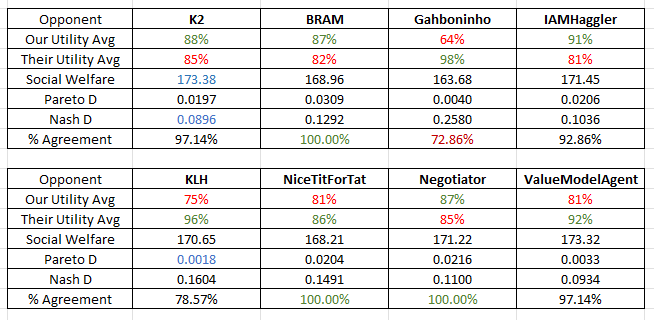
\includegraphics[width=420pt]{table-party.png}
    \caption{Table with average utilities and other values in tests in the party domain.}
    \label{fig:party-vs-agent007}
\end{figure}

Besides the required testing, we did a large scale tournament, with every possible utility on the party domain, against every agent available for the ANAC 2011 competition (but not itself), so we ended up with around \textbf{70 sessions of negotiations} between each agent. As a point of reference, our total average utility for the whole tournament was 0.817, while Gahboninho's, our most challenging opponent, was around 0.884 for a tournament with similar configuration.

It should be highlighted that we managed to always keep the final Pareto and Nash distances reasonably small, which means we are usually ending up on a fair agreement, which is one of the main goals of our agent.

\paragraph{a)}We have evaluated our agent by running several rounds of negotiations against itself, and three other agents (HardHeaded, Gahboninho, and IAMhaggler2011) on the party domain. All the sessions had a deadline of 60 rounds. We started out by letting our agent play against itself for five negotiation sessions, using utility profiles $1$ and $2$. Out of the five sessions, two times no agreement was reached, while the remaining three times the session ended with a result that lies on (or really close to) the Pareto Frontier. However, none of the outcomes were Nash solutions. One interesting thing we noticed is that most of the agreements happen on the exact same point, with utilities $0.878$ and $0.69$ respectively, despite the bids proposed up to that point are always different. An example of those sessions can be seen on Figure \ref{fig:party-vs-agent007}.

\begin{figure}[h!]
    \centering
    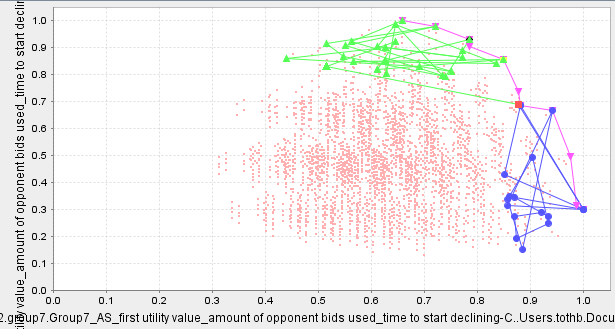
\includegraphics[width=350pt]{party-vs-agent007.PNG}
    \caption{A negotiation session with our agent playing against itself on the party domain with utility profiles 1 and 2.}
    \label{fig:party-vs-agent007}
\end{figure}

To further investigate the phenomenon of always converging on the exact same agreement, we also have run five sessions with utility profiles $3$ and $4$. In all five cases an agreement was reached relatively quickly (with an average of $6.2$ rounds per session, as opposed to $60$ in the first case, which is also the timeout), with all the agreements being different to each other. In this experiment only a single run resulted in a Pareto Efficient agreement, with the other four also being relatively close to the Pareto Frontier (with a distance $<1$). Based on this experiment we can conclude that the previous behavior of always agreeing on the same bid was caused by the specific utility profiles used.

Our agent was also evaluated against three ANAC2011 agents on the party domain, where five sessions were simulated against each of the opponents.
Out of the five games against \textit{HardHeaded} only two games ended with an agreement, with one of those being on the Pareto Frontier, and the other not directly on, but relatively close to it (a distance of about $0.8$). None of the solutions were Nash. 

\textit{Gahboninho} kept offering the same bids all game, completely ignoring the agent's bids. Our agent gradually offered better and better bids, but was generally quite far away from the opponent's even after all $60$ rounds. In the last round our agent finally gave in, and agreed to the offer of the opponent, because it still resulted in a higher utility then finishing the session without an agreement. This however highlights an important shortcoming of our agent, namely that it can easily exploited by simply never changing your preferences. This is a choice we made, since while we lose in a single negotiation session against an stubborn agent, in the long run in a tournament with multiple stubborn agents we will get more agreements, and thus this could lead to a higher average utility.

Against \textit{IAMhaggler2011}, our of the five games ended with an agreement, with all of them laying on the Pareto Frontier. One of these four agreements was also a Nash solution.

\paragraph{b)}In a tournament with the aforementioned three agents on the party domain we found an average utility (excluding the run against ourselves) of $0.900$. After replacing our acceptance strategy by \textit{NiceTitForTat}, the average dropped slightly to $0.884$. Using the acceptance strategy \textit{Accept 10\% best, support uncertainty} performed even worse, with an average utility of $0.747$. Based on these tests we can say that our acceptance strategy is a clear improvement upon already existing methods for our agent, although a lot more testing would be needed to completely confirm that. 

\paragraph{c)}We also compared the performance of our opponent model with the default, \textit{HardHeaded Frequency Model}, by running a tournament with the same parameters as described in section b) above. As opposed to the average utility of $0.900$ of our complete agent, we only achieved an average utility of $0.761$ when using the substitute opponent model. This indicates a clear improvement in our opponent model design, and thus using Bayesian learning was the right choice.

\paragraph{d)}We tested our agent in three domains (\textit{SmartGrid2016}, \textit{ItexvsCypress} and \textit{AmsterdamANAC2011}). In all cases we let our agent play against all of the 2011 agents, with all possible combinations of utility profiles. The sessions had a timeout of 100 rounds.


Agent performance in a tournament on \textit{SmartGrid2016} domain: an average agent utility of 0.733 was reached, with an average opponent utility of 0.808. In 94\% of the sessions ended with an agreement, 70\% ended on the Pareto Frontier.

On \textit{ItexvsCypress} domain the agent got an average utility of 0.472, with  an average opponent utility of 0.734. In 94\% of the sessions an agreement was reached, 75\% of sessions ended on the Pareto Frontier. 

On the \textit{AmsterdamANAC2011} domain our agent got an average utility of 0.692, while the average opponent utility was 0.71. An agreement was reached in 87\% of the sessions, with 67\% on the Pareto Frontier.

\item \textbf{FUTURE PERSPECTIVES / CONCLUSION}

For our agent to be useful in real-life scenarios, not only would it need to be more rigorously tested, but it would need a lot more features so it could perform in those new scenarios. Outside the limitations of Genius, the agent should be able to either write out or speak its bid/counter-bid, and also forcefully exit an auction scenario if the proposed bid is out of our own maximum value. Also, if it were able to learn between multiple negotiation sessions, that would certainly improve its chances, while also making the opponent model much better at understanding the different archetypes of opponents.

If we were to reflect on possible improvements inside the Genius API, however, there is a lot to discuss. Like we mentioned in the agent analysis, one of our shortcomings is that our agents concedes heavily against really hard-headed opponents; that is by choice, our agent would rather get any utility at all, than mimic their behaviour and not reach an agreement. Unfortunately, given the large scale testing we did, we noticed our average utility is much smaller against stubborn opponents (20-25\% smaller), and we also 'lost' against some agents that were more conceding; toning down our concessions and looking for bids slightly better for us, while keeping close to the Pareto frontier would be a priority in future version of this agent.  Also, we have no guarantee that our opponent model is actually a perfect representation of the opponent's preferences, highlighted by the fact that we don't always get agreements when our agents plays against itself; since both of the agents are looking for a good agreement between both parties, it is expected that an agreement close to the Pareto frontier would always be reached. A possible solution for that issue would be to return to our 'discovery' phase in case the our opponent model signals that it's weights are drastically changing again. That way, we would be more resilient against unpredictable agents.

\end{enumerate}

\bibliographystyle{apalike}
\bibliography{ref}

\end{document}